\documentclass[border=10pt]{standalone}
\usepackage{tikz}

\begin{document}
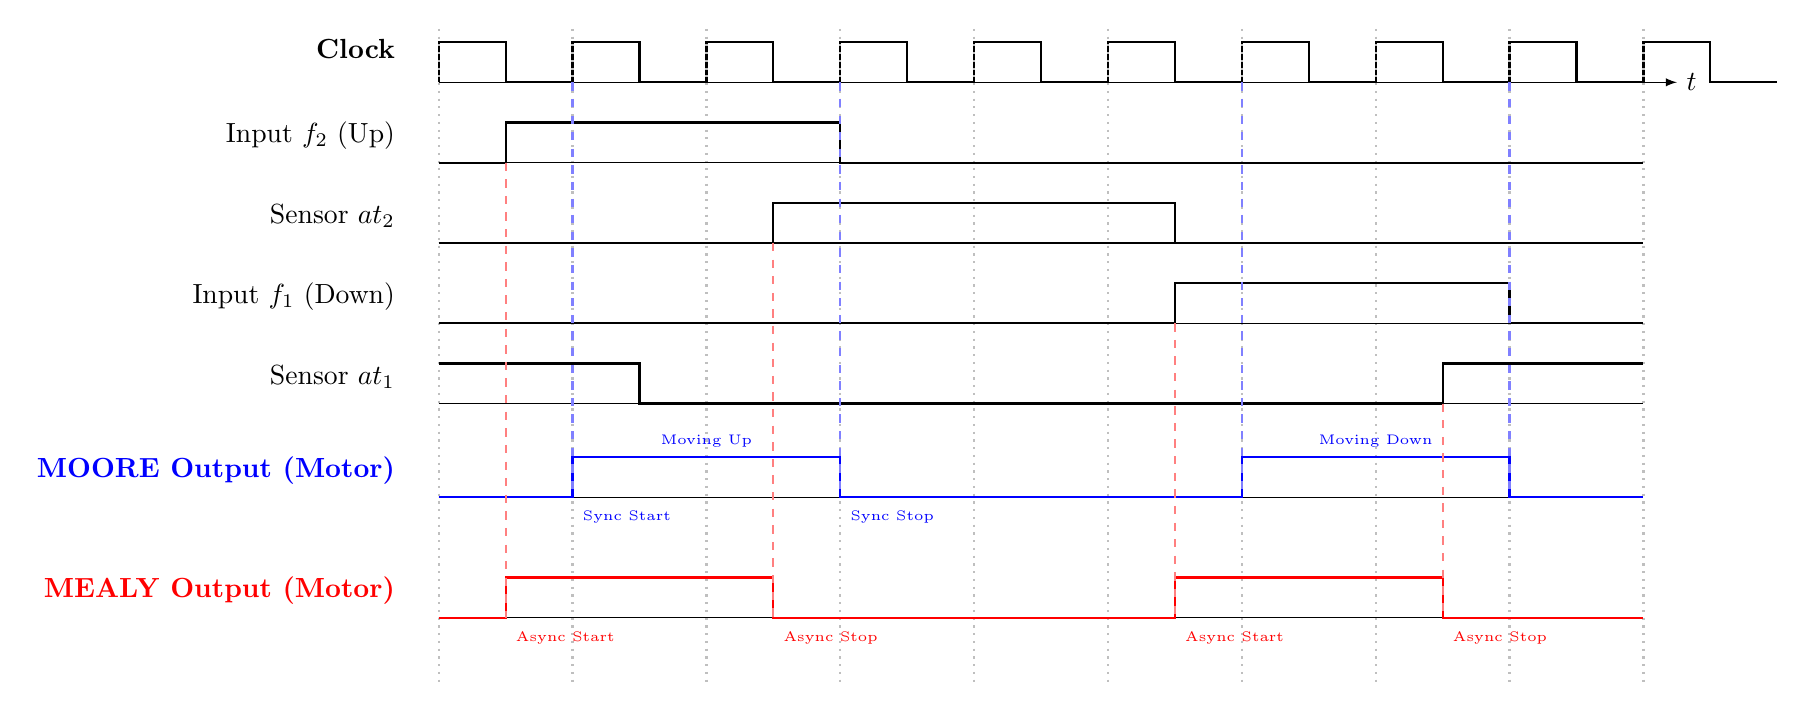
\begin{tikzpicture}[thick, >=latex, scale=0.85]
  % Define coordinates and heights
  \def\h{0.6}
  \def\w{1.5}
  \def\MAXT{18}
  
  % --- Grid helpers ---
  %\draw[step=1, gray!20, thin] (0,0) grid (\MAXT, 10);
  
  % --- Clock ---
  \node[left, font=\bfseries] at (-0.5, 9.5) {Clock};
  \draw[thin, ->] (0, 9) -- (\MAXT+0.5, 9) node[right] {$t$};
  \foreach \i in {0,...,9} {
    \draw (\i*2, 9) -- ++(0, \h) -- ++(1, 0) -- ++(0, -\h) -- ++(1, 0);
    \draw[dotted, gray!50] (\i*2, 9.8) -- (\i*2, 0); % Vertical reference lines (Rising Edge)
  }
  
  % --- Inputs ---
  
  % f2 (Call Up)
  \node[left] at (-0.5, 8.2) {Input $f_2$ (Up)};
  \draw[thin] (0, 7.8) -- (\MAXT, 7.8);
  % Press f2 at t=1, release after arrival (say t=6)
  \draw[thick] (0, 7.8) -- (1, 7.8) -- (1, 7.8+\h) -- (6, 7.8+\h) -- (6, 7.8) -- (\MAXT, 7.8);
  
  % at2 (Sensor Floor 2)
  \node[left] at (-0.5, 7.0) {Sensor $at_2$};
  \draw[thin] (0, 6.6) -- (\MAXT, 6.6);
  % Arrives at t=5 (mid-cycle), stays until leaves
  % Leaves when moving down later
  \draw[thick] (0, 6.6) -- (5, 6.6) -- (5, 6.6+\h) -- (11, 6.6+\h) -- (11, 6.6) -- (\MAXT, 6.6);
  
  % f1 (Call Down)
  \node[left] at (-0.5, 5.8) {Input $f_1$ (Down)};
  \draw[thin] (0, 5.4) -- (\MAXT, 5.4);
  % Press f1 at t=11, release after arrival (say t=16)
  \draw[thick] (0, 5.4) -- (11, 5.4) -- (11, 5.4+\h) -- (16, 5.4+\h) -- (16, 5.4) -- (\MAXT, 5.4);
  
  % at1 (Sensor Floor 1)
  \node[left] at (-0.5, 4.6) {Sensor $at_1$};
  \draw[thin] (0, 4.2) -- (\MAXT, 4.2);
  % Initially at floor 1 (High). Leaves when starts up (t=2 approx). Returns at t=15.
  \draw[thick] (0, 4.2+\h) -- (3, 4.2+\h) -- (3, 4.2) -- (15, 4.2) -- (15, 4.2+\h) -- (\MAXT, 4.2+\h);
  
  
  % --- MOORE Side ---
  \node[left, font=\bfseries, blue] at (-0.5, 3.2) {MOORE Output (Motor)};
  \draw[thin] (0, 2.8) -- (\MAXT, 2.8);
  
  % Logic: 
  % 1. Start Up: f2=1 at t=1. Clock edge t=2 -> State 11 (Up). Motor=1.
  % 2. Stop Up: at2=1 at t=5. Clock edge t=6 -> State 10 (Floor 2). Motor=0.
  % 3. Start Down: f1=1 at t=10. Clock edge t=12 -> State 01 (Down). Motor=1. (Wait, edge is at 10, 12, 14. f1 at 10. If setup time met, changes at 12? No, input change at 10 mid cycle? 
  % Let's align inputs away from edges to be clear.
  % f1 at t=10? Edge is at 10. Let's start f1 at t=9.
  % Adjusted f1 above to t=10. Edges are 0, 2, 4, 6, 8, 10, 12, 14, 16, 18.
  % If f1 is sync with edge, ambiguous. Let's move f1 to t=11 (mid cycle).
  % Edge at t=12 captures f1=1. State -> 01 (Down). Output -> 1.
  % 4. Stop Down: at1=1 at t=14. Edge at t=16? No, at1 at t=14 (edge). Let's move at1 to t=15 (mid cycle).
  % Edge at t=16 captures at1=1. State -> 00 (Floor 1). Output -> 0.
  
  % Let's refine Timing of Inputs to be clearly async (mid-cycle):
  % f2: t=1. Edge t=2. Moore Start t=2.
  % at2: t=5. Edge t=6. Moore Stop t=6.
  % f1: t=11. Edge t=12. Moore Start t=12.
  % at1: t=15. Edge t=16. Moore Stop t=16.
  
  \draw[blue, thick] (0, 2.8) -- (2, 2.8) -- (2, 2.8+\h) -- (6, 2.8+\h) -- (6, 2.8) -- (12, 2.8) -- (12, 2.8+\h) -- (16, 2.8+\h) -- (16, 2.8) -- (\MAXT, 2.8);
  
  % Add Labels
  \node[above, blue, font=\tiny] at (4, 2.8+\h) {Moving Up};
  \node[above, blue, font=\tiny] at (14, 2.8+\h) {Moving Down};
  \node[right, blue, font=\tiny] at (2, 2.5) {Sync Start};
  \node[right, blue, font=\tiny] at (6, 2.5) {Sync Stop};
  
  
  % --- MEALY Side ---
  \node[left, font=\bfseries, red] at (-0.5, 1.4) {MEALY Output (Motor)};
  \draw[thin] (0, 1.0) -- (\MAXT, 1.0);
  
  % Logic: Output = (Up Logic) OR (Down Logic)
  % Up Logic: !Q * f2 (Start) ... wait, standard Mealy:
  % Floor 1: If f2 -> Go Up. (Immediate).
  % Arrive Floor 2: If at2 -> Stop (Next State Floor 2).
  % Actually Mealy output depends on Input.
  % Floor 1 State: Input f2 -> Output 1.
  % Floor 1 State: Input f2 & at2 -> Output ??
  % Usually Mealy defines output on transition.
  % Trans: Floor 1 -> Floor 2 (Condition f2 & at2).Output?
  % If we look at the Mealy diagram in lecture:
  % Floor 1 Loop: f2=1, at2=0 -> Out=1.
  % Transitions to Floor 2 when at2=1. during that transition, does it output 1 or 0?
  % Diagram (Fig 8-10): Loop on Floor 1 (f2=1, at2=0 / 11) -> Output 11 (Motor On).
  % Edge to Floor 2 (f2=1, at2=1 / 10) -> Output 10 (Motor Off? No, wait).
  % The edge label is Input/Output.
  % Loop: f2=1, at2=0 / 11 (Go=1).
  % Edge: f2=1, at2=1 / 10 (Go=1?).
  % Wait, if it outputs 1 during transition, it stops only AFTER entering Floor 2 state?
  % Mealy Output valid for the *duration* of the input condition in that state.
  % So while in Floor 1: if f2=1 and at2=0, Go=1.
  % When at2 becomes 1 (at t=5): Condition becomes f2=1, at2=1.
  % Edge label for (f2=1, at2=1) is "10" (Go=1, Led=0).
  % Wait, if go=1 when arriving, it overshoots?
  % Let's look at the Mealy Table in Lecture 8.
  % PS=0 (Floor 1). Input: f2=1, at2=1 -> NS=1. Out=10 (Led=1, Go=0).
  % Ah! The table says Go=0 when arriving!
  % So Output becomes 0 *immediately* when at2=1.
  
  % So:
  % Start Up: f2=1 at t=1. Go=1 immediately.
  % Stop Up: at2=1 at t=5. Go=0 immediately.
  % Start Down: f1=1 at t=11. Go=1 immediately.
  % Stop Down: at1=1 at t=15. Go=0 immediately.
  
  \draw[red, thick] (0, 1.0) 
    -- (1, 1.0) -- (1, 1.0+\h) -- (5, 1.0+\h) -- (5, 1.0) % Up Leg
    -- (11, 1.0) -- (11, 1.0+\h) -- (15, 1.0+\h) -- (15, 1.0) % Down Leg
    -- (\MAXT, 1.0);
    
  \node[right, red, font=\tiny] at (1, 0.7) {Async Start};
  \node[right, red, font=\tiny] at (5, 0.7) {Async Stop};
  \node[right, red, font=\tiny] at (11, 0.7) {Async Start};
  \node[right, red, font=\tiny] at (15, 0.7) {Async Stop};
  
  % vertical dashed lines for key events
  \draw[dashed, red!50] (1, 7.8) -- (1, 1.0); % f2 start
  \draw[dashed, blue!50] (2, 9.0) -- (2, 2.8); % Clock edge
  
  \draw[dashed, red!50] (5, 6.6) -- (5, 1.0); % at2 start
  \draw[dashed, blue!50] (6, 9.0) -- (6, 2.8); % Clock edge
  
  \draw[dashed, red!50] (11, 5.4) -- (11, 1.0); % f1 start
  \draw[dashed, blue!50] (12, 9.0) -- (12, 2.8); % Clock edge
  
  \draw[dashed, red!50] (15, 4.2) -- (15, 1.0); % at1 start
  \draw[dashed, blue!50] (16, 9.0) -- (16, 2.8); % Clock edge

\end{tikzpicture}
\end{document}
